\documentclass{article}%
\usepackage[T1]{fontenc}%
\usepackage[utf8]{inputenc}%
\usepackage{lmodern}%
\usepackage{textcomp}%
\usepackage{lastpage}%
\usepackage{geometry}%
\geometry{left=2.5cm,top=1.5cm}%

\usepackage[table, dvipsnames]{xcolor}
%\usepackage[usenames]{color}
\usepackage{stmaryrd}
%\usepackage{array}
\usepackage{xfp}
\usepackage{fp}
\usepackage{pgf}
\usepackage{graphicx}
\usepackage{subfigure}
\usepackage{mathtools}
\usepackage[natbibapa]{apacite}
\bibliographystyle{apacite}
\graphicspath{ {images/} }
\usepackage{vmargin}
\usepackage{amsmath}
\usepackage{circuitikz}
\usepackage{tikz}
\usepackage{tocloft}
\usetikzlibrary{calc}
\usetikzlibrary{arrows}

\usepackage{pgfplots}
\pgfplotsset{compat=1.10}
\usepgfplotslibrary{fillbetween}
\usetikzlibrary{patterns}


\usepackage{units}
\usepackage{setspace}
\usepackage{multicol}
\usepackage{multirow}
\usepackage{colortbl}
\usepackage{array}
\usepackage{booktabs}
\usepackage{caption}
\usepackage{amssymb}
\usepackage{amsfonts}
\usepackage{amsthm}
\usepackage{amsmath,yhmath}
\usepackage{geometry}
%\usepackage{subcaption}
\usepackage{graphicx}
\usepackage[export]{adjustbox}
\usepackage[framemethod=tikz]{mdframed}
\usepackage{lipsum}
\usepackage{tcolorbox}
\usepackage{tocloft}
\usepackage{fancyhdr}
\usepackage{float}
%\usepackage[colorlinks,citecolor=red]{hyperref}
%\usepackage{}
%\newtcolorbox{mybox2}{colback=red!5!white,colframe=red!75!black,width=0.85\textwidth}
\newtcolorbox{mybox2}[1]{colback=gray!5!white,colframe=cyan!75!black,fonttitle=\bfseries,title=#1}

\newtcolorbox{mybox3}[1]{colback=gray!5!white,colframe=Maroon!75!black,fonttitle=\bfseries,title=#1}

\newtcolorbox{mybox4}[1]{colback=gray!5!white,colframe=LimeGreen!75!black,fonttitle=\bfseries,title=#1}


\newcommand{\listequationsname}{\Large Lista de ecuaciones}
\newlistof{myequations}{equ}{\listequationsname}
\newcommand{\myequations}[1]{%
\addcontentsline{equ}{myequations}{Ecuación\hspace{0.3em}\protect\numberline{\theequation}#1}\par}
\setlength{\cftmyequationsnumwidth}{1.75em}
\setlength{\cftmyequationsindent}{1.5em}
\addtocontents{equ}{~\hfill\textbf{Página}\par}


\definecolor{mycolor}{rgb}{0.122, 0.435, 0.698}
%\captionsetup[table]{name=Tabla}
%\usepackage{bigstrut}
\setpapersize{A4}
\setmargins{2.5cm}       % margen izquierdo
{1.5cm}                        % margen superior
{16.5cm}                      % anchura del texto
{23.42cm}                    % altura del texto
{10pt}                           % altura de los encabezados
{1cm}                           % espacio entre el texto y los encabezados
{0pt}                             % altura del pie de página
{2cm}                           % espacio entre el texto y el pie de página
\usepackage{diagbox}
\usepackage{slashbox}
\usepackage{url}


\renewcommand{\listfigurename}{Lista de Figuras}
\renewcommand{\listtablename}{Lista de Tablas}
\renewcommand{\baselinestretch}{1.5}
\renewcommand{\abstractname}{Resumen}
\renewcommand{\figurename}{Figura}
\renewcommand{\contentsname}{\underline{Contenido}}
\renewcommand{\tablename}{Tabla}
\renewcommand{\cftfigfont}{Figura }
\renewcommand{\cfttabfont}{Tabla }
\addtocontents{toc}{~\hfill\textbf{Página}\par}
\addtocontents{lot}{~\hfill\textbf{Página}\par}
\addtocontents{lof}{~\hfill\textbf{Página}\par}
\providecommand{\keywords}[1]
{
  \textbf{\text{Palabras clave: }} #1
}

\title{\textbf{MEMORIA DE CALCULO ESTRUCTURAL}}
\author{VIVIENDA MULTIFAMILIAR}
\date{Junio 06, 2022}
\usepackage[hidelinks]{hyperref}

\pagestyle{fancy}
\fancyhf{}
% \rhead{\includegraphics[trim={0 5cm 0 2.2cm},clip,width=27mm]{PORTADA (4).png}}
\lhead{MEMORIA DE CALCULO}
%\rfoot{Página\ \thepage\ de \numpages}
\lfoot{Realizado por: \textit{Alexis Pompilla Yábar}}
\cfoot{}
\renewcommand{\headrulewidth}{0.4pt}
\renewcommand{\footrulewidth}{0.4pt}
\rfoot{Página\ \thepage}
%\AtBeginDocument{\addtocontents{toc}{\protect\thispagestyle{empty}}} 


%%%%%%%%%%%%%%%%%%%%%%%%%%%%%%%%%%%%%%%%%%%%%%%%%%%%%%%%%%%%%%%%%%%%%%%%%%%%%%%%%%%%%%%%%%%%%%%%%%%%%%%%%%%%
%%%%%%%%%%%%%%%%%%%%%%%%                        Nuevos comandos         %%%%%%%%%%%%%%%%%%%%%%%%%%%%%%%%%%%%
\setlength{\parindent}{0pt} % sin sangría
%\renewcommand{\multirowsetup}{\centering}
%\newlength{\LL}\settowidth{\LL}{texto}

%% -------------------------------------------------------------------------------------------------------- %%
%%                                          ECUACIONES                                                      %%
%% -------------------------------------------------------------------------------------------------------- %%

\usepackage{xargs}


\newcommandx{\mycommandEC}[4][1=a, 2=b, 3=c, 4=]{%
	% Cuerpo del comando
	% Aquí puedes utilizar los argumentos #1, #2 y #3
	%\begin{align#4}
		x_{1, 2} &= \dfrac{- #2 \pm \sqrt{#2^2 - 4 \cdot #1 \cdot #3} }{2 \cdot #1} 		%\tag{A}
	%\end{align#4}
}

% Longitud de desarrollo %Varibles db, fy, f'c
\newcommandx{\Ldi}[3][1=d_b, 2=f_y, 3=f'_c]{0.08 \cdot #1 \cdot \dfrac{#2}{\sqrt{#3}}}
\newcommandx{\Ldii}[2][1=d_b, 2=f_y]{0.004 \cdot #1 \cdot #2}

% d = max(ld1, ld2)
\newcommandx{\ddd}[2][1=L_{d1}, 2=L_{d2}]{\max(#1, #2)}

% hz = d + 0.1m
\newcommandx{\hz}[1][1=d]{d + 0.1m}

% Capacidad portante neta del terreno
% Variables: σn = σt - γc·hz - γm·hs - γc·hp - S/C_piso
\newcommandx{\qn}[7][1=\sigma_t, 2=\gamma_c, 3=h_z, 4=\gamma_m, 5=h_s, 6=h_p, 7=S/C_{piso}]{#1 - #2 \cdot #3 - #4\cdot#5 - #2\cdot#6 - #7}

% Área tentativa % Variables: Pservicio, σn
\newcommandx{\AreaTentativa}[2][1=P_{servicio}, 2=\sigma_n]{\dfrac{#1}{#2}}
 
% Dimensiones de la zapata L y B
% Variables: At, c1, c2
\newcommandx{\LongitudZapL}[3][1=A_t, 2=c_1, 3=c_2]{\sqrt{#1} + \dfrac{#2 - #3}{2}} %Para L
\newcommandx{\LongitudZapB}[3][1=A_t, 2=c_1, 3=c_2]{\sqrt{#1} - \dfrac{#2 - #3}{2}} %Para B
\newcommandx{\Area}[2][1=L, 2=B]{#1 \cdot #2}

% Verificación de zapatas con cargas y momentos biaxiales
% variables: Pultima, Area(A), Mx, Vx, Iyy + My, Vy, Ixx
\newcommandx{\EcPresiones}[8][1=P_{ultima}, 2=A, 3=M_x, 4=V_x, 5=I_{yy}, 6=M_y, 7=V_y, 8=I_{xx}]{\sigma_{1,2,3,4} = \dfrac{#1}{#2} \pm \dfrac{#3\cdot#4}{#5} \pm \dfrac{#6\cdot#7}{#8}}

% Verificación de corte por punzonamiento
% Sección crítica bo, variables: c1, c2, d
\newcommandx{\SeccCriticaP}[3][1=c_1, 2=c_2, 3=d]{2(#1 + #3) + 2(#2 + #3)}
% Area tributaria, variables: c1, c2, d
\newcommandx{\AreaTributariaP}[3][1=c_1, 2=c_2, 3=d]{(#1 + #3)\cdot(#2 + #3)}

% Cortante de diseño por corte-punzonamiento
% Variables: σu, A, Ao
\newcommandx{\VuPunzonamiento}[3][1=\sigma_u, 2=A, 3=A_o]{#1 \cdot (#2 - #3)}

% Verificación cortante por punzonamiento (las 3 verificaciones)
% Variables: σ=0.85, f'c, bo, d, αs, β
\newcommandx{\VcPunzonamientoi}[4][1=f'_c, 2=b_o, 3=d, 4=\beta]{0.85 \cdot (0.17 \left( 1 + \dfrac{2}{#4} \right) \sqrt{#1}\cdot #2 \cdot #3)}

\newcommandx{\VcPunzonamientoii}[5][1=f'_c, 2=b_o, 3=d, 4=\beta, 5=\alpha_s]{0.85 \cdot ( 0.083 \left( \dfrac{#5 \cdot #3}{#2} + 2\right) \sqrt{#1}\cdot #2 \cdot #3)}

\newcommandx{\VcPunzonamientoiii}[3][1=f'_c, 2=b_o, 3=d]{0.85 \cdot (0.33 \cdot \sqrt{#1} \cdot #2 \cdot #3)}


% Cortante de diseño por flexion
% Variables: σu, B, c, d
\newcommandx{\VuFlexion}[4][1=\sigma_u, 2=B, 3=c, 4=d]{#1 \cdot #2 \cdot (#3 - #4)}

% Verificación cortante por corte-flexion
% Variables: σ=0.85, f'c, B, d
\newcommandx{\VcFlexion}[3][1=f'_c, 2=B, 3=d]{0.85 \cdot 0.17 \cdot \sqrt{#1} \cdot #2 \cdot #3}

% Cálculo de acero por flexión
% Variables: σu, Lv=, B=prof de la zapata
\newcommandx{\MomUltimoi}[3][1=\sigma_u, 2=L_v, 3=B]{\dfrac{#1 \cdot (#2)^2 \cdot #3}{2}}

% Variables: Mu, φ, B, d, f'c, %%w
\newcommandx{\MomUltimoii}[5][1=M_u, 2=\phi, 3=B, 4=d, 5=f'c]{#1 = #2 (#3)(#4^2)(#5)(w)(1 - 0.59 \cdot w)}

% Cálculo del área de acero
% Variables: w, b, d, f'c, fy
\newcommandx{\AreaAcero}[5][1=w, 2=b, 3=d, 4=f'_c, 5=f_y]{\dfrac{#1 \cdot #2 \cdot #3 \cdot #4}{#5}}

% Área de acero mínimo
% Variables: b, h
\newcommandx{\AreaAceroMin}[2][1=b, 2=h]{0.0018 \cdot #1 \cdot #2}
%
%
%
%
\begin{document}%
\normalsize%

\normalsize%

%\setlength{\abovedisplayskip}{0pt}
%\setlength{\belowdisplayskip}{0pt}
%\setlength{\abovedisplayshortskip}{0pt}
%\setlength{\belowdisplayshortskip}{0pt}
\maketitle
% \begin{figure}[h!]
%     \centering
%     \includegraphics[scale=0.75]{IMAGENES/r2.png}
%     \label{fig:my_label}
% \end{figure}
\thispagestyle{empty}
\newpage

\clearpage                       % Otherwise \pagestyle affects the previous page.
{                                % Enclosed in braces so that re-definition is temporary.
  \pagestyle{empty}              % Removes numbers from middle pages.
  \fancypagestyle{plain}         % Re-definition removes numbers from first page.
  {
    \fancyhf{}%                       % Clear all header and footer fields.
    \renewcommand{\headrulewidth}{0pt}% Clear rules (remove these two lines if not desired).
    \renewcommand{\footrulewidth}{0pt}%
  }
    \begin{spacing}{1.35}
    \tableofcontents
  \end{spacing}
  \thispagestyle{empty}  
  \listoffigures
\newpage
\listoftables
  \thispagestyle{empty} 
% Removes numbers from last page.
}


%\listofmyequations
%\header{Realizado por: Alexis Pompilla Yábar}{}{}
\newpage


\subsection{Diseño de la cimentación}
Se presentaran las consideraciones para el dimensionamiento de la cimentación, control de presiones y el cálculo del refuerzo con las verificaciones necesarias en concreto armado.\\
Se asumen dos hipótesis básicas:
\begin{enumerate}
    \item El suelo es homogéneo, elástico y aislado del suelo circundante.
    \item Considerar la flexibilidad de la Cimentación y del suelo.
\end{enumerate}

\subsubsection{Modelamiento}
El modelo matemático simple que se usa en la practica consiste en incluir la flexibilidad del suelo a través de módulos de subrasante, el modelo más conocido es la solución de Winkler.\\
Es un modelo aproximado que se propuso en 1867, el cual sirve para resolver fundaciones sobre medios elásticos. Este método considera el suelo como un lecho de resortes. La presión de contacto queda definida por el producto de la rigidez elástica del resorte y el asentamiento que se ha producido en él debido a las cargas que actúan.\\

% \begin{figure}[h!]
%     \centering
%     \caption{Modelamiento de la cimentación}
%     \includegraphics[trim={0 0.5cm 0 0},clip,scale=0.6]{IMAGENES/safe2.png}
%     %\caption*{\small Fuente: \it \cite{empuje}}
%     \label{atrans}
% \end{figure} 
\newpage
En su tesis de maestría el ingeniero Nelson Morrison recopila varios estudios anteriormente realizados que relacionan directamente el módulo de subrasante con la capacidad admisible del suelo, el cual es válido para un área y NO necesita ser modificado a las dimensiones de la cimentación.

% \begin{figure}[h!]
%     \centering
%     \caption{Coeficientes de Winkler}
%     \includegraphics[scale=1]{IMAGENES/safe3.PNG}
%     %\caption*{\small Fuente: \it \cite{empuje}}
%     \label{atrans}
% \end{figure} 

Cabe resaltar que para el diseño de fundaciones SAFE usa el Modelo de Winkler , el cual se resuelve a través del método de los elementos finitos FEM, usando elementos línea, áreas y resorte.\\
Structural Analysis by Finite Elements (SAFE), es un software creado por la empresa Computers and Structures, Inc. (CSI) , el cual sirve para diseñar sistemas de pisos ( Losas y Vigas) y Sistemas de Fundaciones.
% \begin{figure}[h!]
%     \centering
%     \caption{SAFE}
%     \includegraphics[scale=0.3]{IMAGENES/33.jpg}
%     %\caption*{\small Fuente: \it \cite{empuje}}
%     \label{atrans}
% \end{figure} 

\subsubsection{Tipología de la cimentación}
Se proyectan zapatas aisladas, zapatas combinadas y plateas parciales, debido a la presencia de las edificaciones vecinas las cimentaciones resultan excéntricas en 3 lados del edificio por lo que se hace uso de vigas rígidas de cimentación para controlar los momentos producto de la excentricidad de la carga axial. Tales vigas son diseñadas solo para tomar los momentos y uniformizar las presiones en la cimentación y no es diseñada para soportar fuerzas inducidas por la presión del suelo, por lo que debe ser aislada del suelo adecuadamente.\\
El peralte de la cimentación adoptado es el requerido para las solicitaciones de corte y/o punzonamiento en la cimentación, así como para asegurar el desarrollo del refuerzo que llega de las columnas y muros.\\
En las zapatas aisladas no existe momentos que traccionen la cara superior de la zapata por lo que no es necesario colocar refuerzo superior, sin embargo en las zapatas combinadas o cuando se colocan vigas de conexión si existen momento positivo y negativo, por lo que es necesario colocar doble malla.

\subsubsection{Exportación de cargas de ETABS a SAFE}
Debido a que los resultados del análisis modal espectral son productos de una combinación se pierde el signo en las fuerzas, para un análisis racional se exporto las cargas de los modos principales en ambas direcciones escalando sus valores proporcionalmente al valor los momentos totales en la base que se generan a partir de las fueras sísmicas de diseño.

\subsubsection{Predimensionamiento}

Se dimensiono preliminarmente considerando cargas en servicio (D+L) con un 90\% de la capacidad portante para tener holgura cuando se verifica con cargas sísmicas, posteriormente estas dimensiones se corrigieron después del análisis.\\
Para las zapatas combinadas se trató de hacer coincidir el centro de gravedad de la zapata con el de las cargas para el caso de cargas gravitacionales (D+L), adicionalmente en todos los casos se dimensiono tratando de tener volados iguales en ambas direcciones para uniformizar el diseño en concreto armado.\\
Después de realizar un análisis iterativo se obtiene las áreas de cimentación mostradas en la figura  para no superar la presión admisible tanto para cargas de gravedad y sísmicas. 

\subsubsection{Control de presiones}
% \begin{theo}[15.2.4 y 15.2.5 de la norma E-060:]{thm:ca1}
% 15.2.4 Se podrá considerar un incremento del 30\% en el valor de la presión admisible del suelo para los estados de cargas en los que intervengan cargas temporales, tales como sismo o viento.\\
% 15.2.5 Para determinar los esfuerzos en el suelo o las fuerzas en pilotes, las acciones sísmicas podrán reducirse al 80\% de los valores provenientes del análisis, ya que las solicitaciones sísmicas especificadas en la NTE E.030 Diseño Sismorresistente están especificadas al nivel de resistencia de la estructura.
% \end{theo}
\newpage
\noindent Por lo tanto las combinaciones para el control de presiones en condiciones de servicio sera:
\begin{center}
    S1= CM + CV\\
    S2= ( CM+CV + 0.8 SX )/1.3\\
    S3= ( CM+CV - 0.8 SX )/1.3\\
    S4= ( CM+CV + 0.8 SY )/1.3\\
    S5= ( CM+CV - 0.8 SY )/1.3 
\end{center}
\noindent 
Donde:\\
CM: Carga muerta en servicio\\
CV: Carga viva en servicio\\
SX: Carga sísmica en dirección X\\
SY: Carga sísmica en dirección Y\\

% \begin{figure}[h!]
%     \centering
%     \subfigure[Sin vigas de conexión]{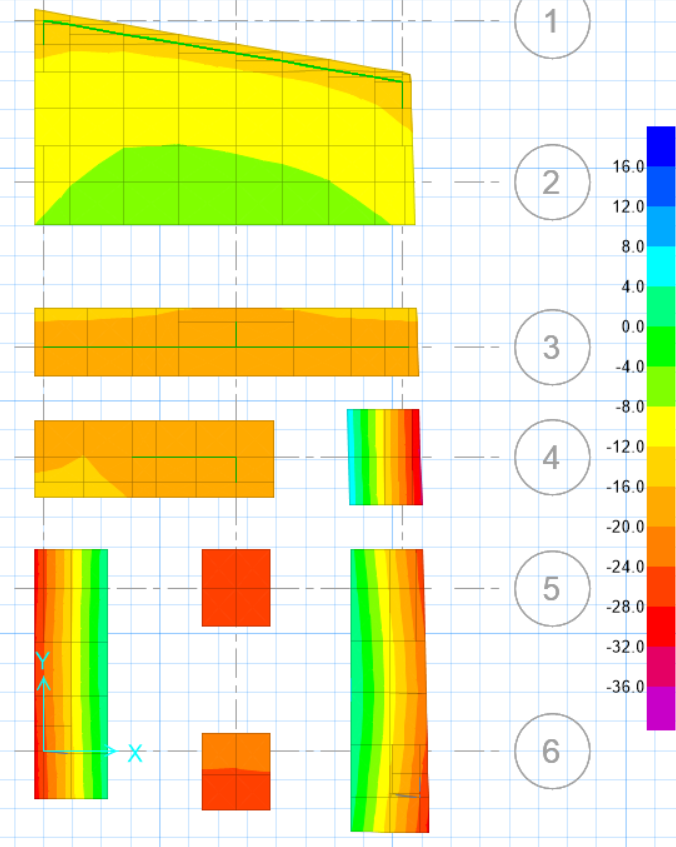
\includegraphics[width=70mm]{IMAGENES/wvc.PNG}}\hspace{10mm}
%     \subfigure[Con vigas de conexión de 30x70]{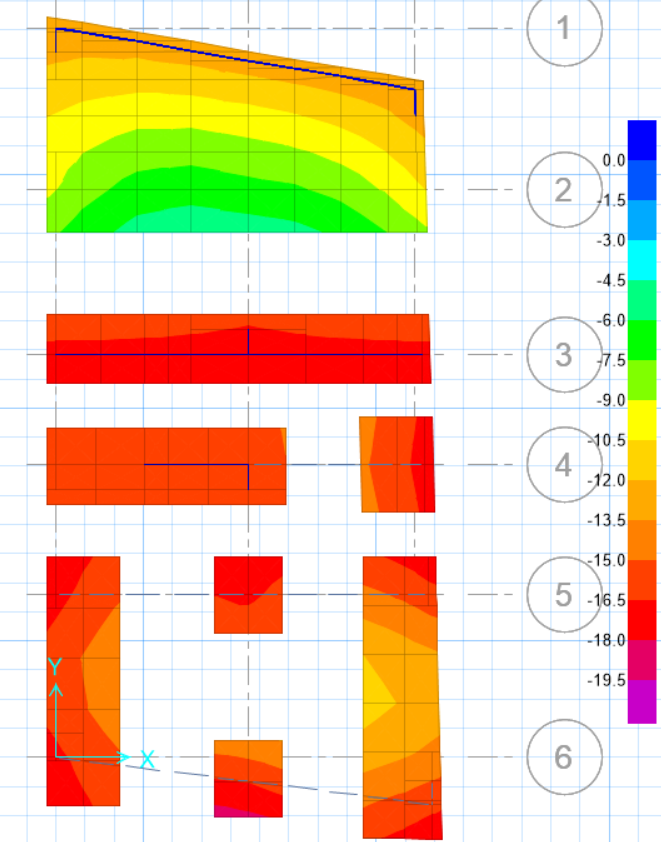
\includegraphics[width=70mm]{IMAGENES/co1.PNG}}
%     \caption{Presiones para la combinación D+L }
%     \label{corw}
% \end{figure}
\newpage
% \begin{figure}[h!]
%     \centering
%     \subfigure[D+L+SX]{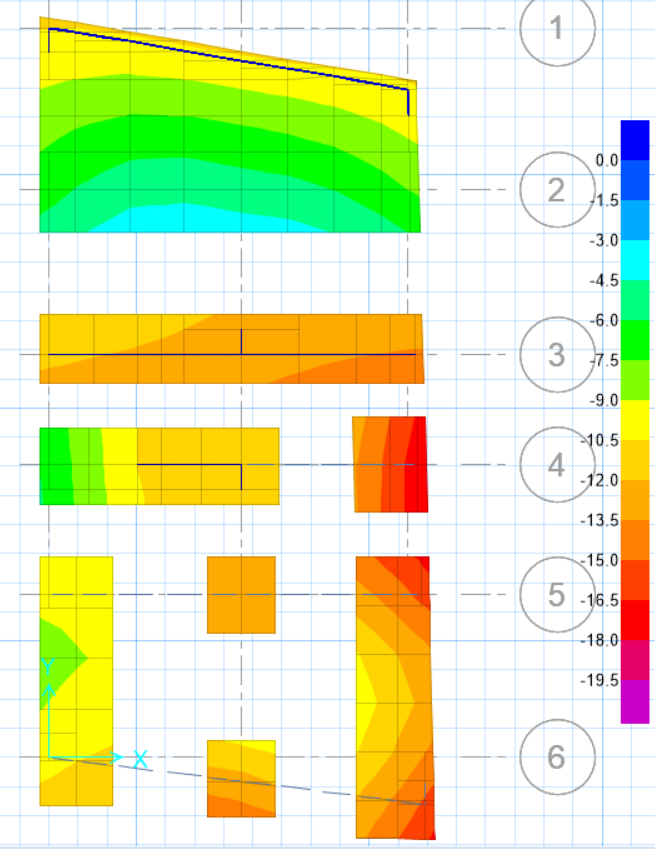
\includegraphics[width=70mm]{IMAGENES/co2.PNG}}\hspace{10mm}
%     \subfigure[D+L-SX]{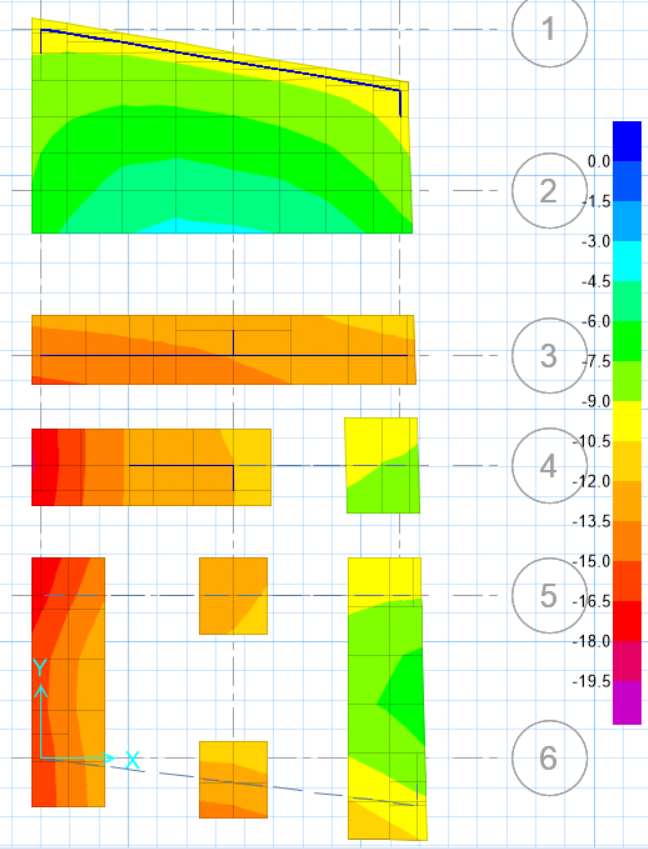
\includegraphics[width=70mm]{IMAGENES/co3.PNG}}
%     \caption{Presiones para la combinación con sismo en X}
%     \label{corw}
% \end{figure}

% \begin{figure}[h!]
%     \centering
%     \subfigure[D+L+SY]{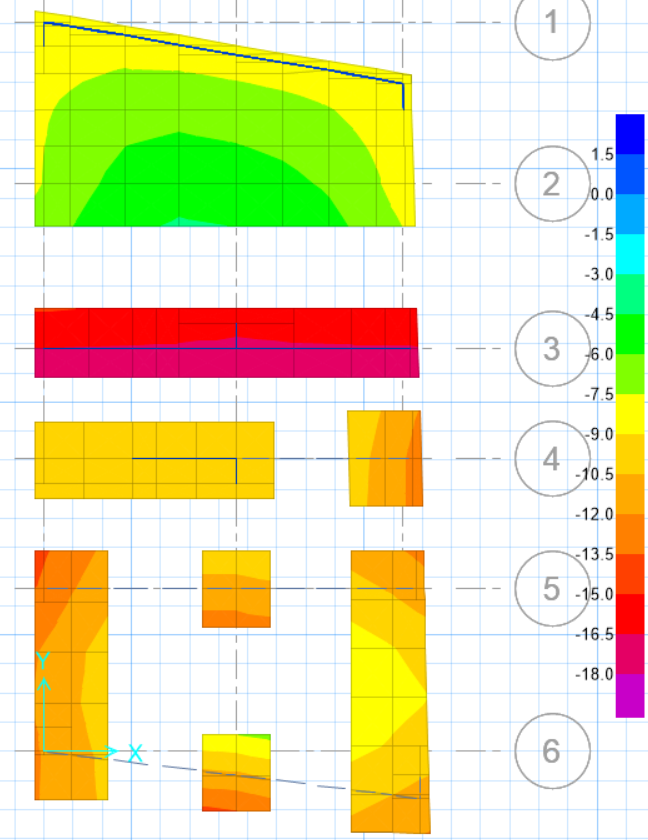
\includegraphics[width=70mm]{IMAGENES/co4.PNG}}\hspace{10mm}
%     \subfigure[D+L-SY]{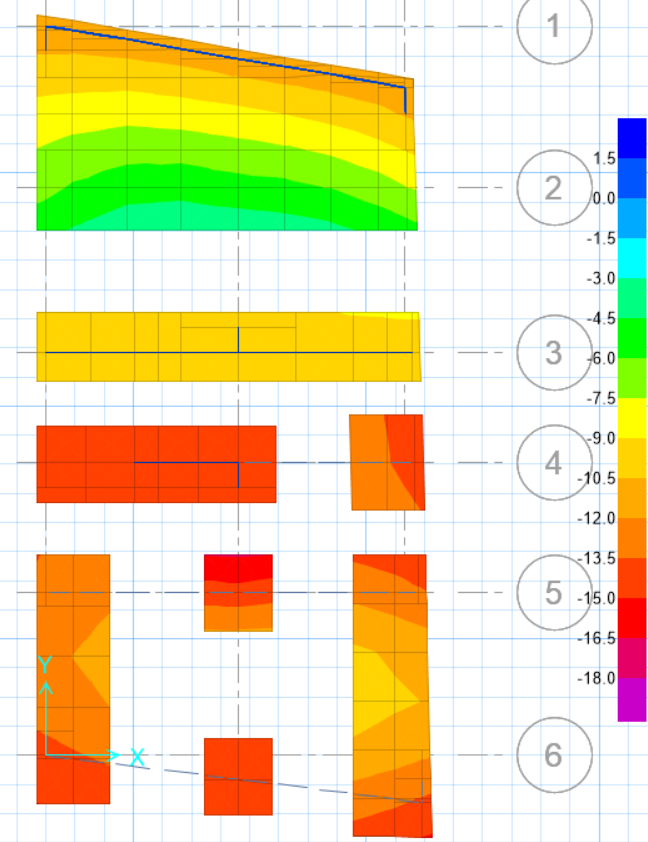
\includegraphics[width=70mm]{IMAGENES/co5.PNG}}
%     \caption{Presiones para la combinación con sismo en Y}
%     \label{corw}
% \end{figure}
\noindent
La capacidad portante admisible del terreno a -2.8m donde se cimienta la parte frontal del edifico es de $1.82\mathrm{~kg/cm^2} $.\\
En la parte posterior a una cota de +0.50m la capacidad portante admisible del terreno es $1.42\mathrm{~kg/cm^2}$.\\
En todos los casos se cumple con la condición: $q_{u}\leq q_{n}$, siendo el caso mas critico la combinación de cargas gravitacionales dado que las cargas sísmicas se reducen considerablemente debido a lo mencionado en los artículos 15.2.4 y 15.2.5 de la \cite{E-060}.\\
Las dimensiones finales se muestran en la figura \ref{dim}:
% \begin{figure}[h!]
%     \centering
%     \caption{Dimensiones de la cimentación}
%     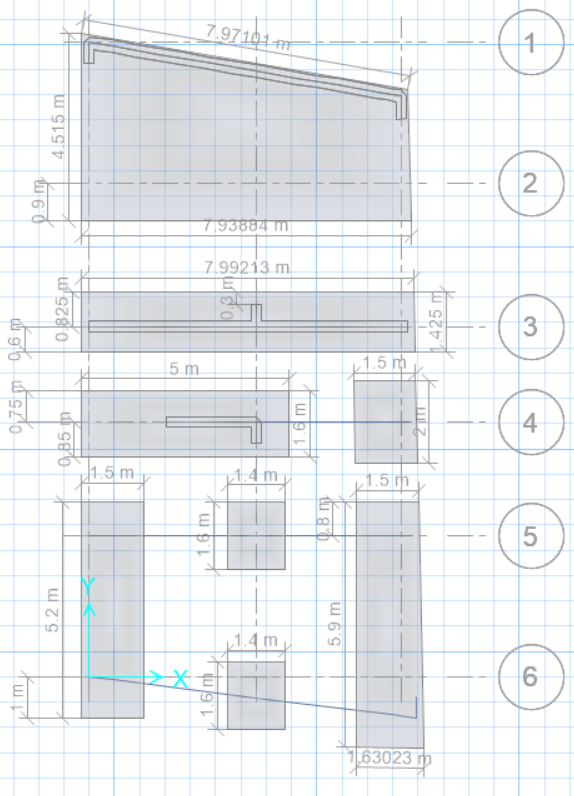
\includegraphics[scale=0.9]{IMAGENES/dim.PNG}
%     %\caption*{\small Fuente: \it \cite{empuje}}
%     \label{dim}
% \end{figure} 

\newpage
\subsubsection{Diseño en concreto armado}
\noindent 
Según el articulo 10.5.4 la cuantía mínima en zapatas sera de 0.0018, y cuando el refuerzo se distribuya en 2 capas la cuantía mínima en la cara en tracción sera 0.0012.\\



\newpage
\section{Diseño de la Cimentación}

\subsection{Diseño de Zapata Aislada}

%% ------------------------------------------------------------------------------------
%%                      DEFINICIÓN DE VARIABLES                                         
%% ------------------------------------------------------------------------------------
\FPset\plosa{0.3} %peso de losa por m2
\FPset\alosa{3.2}
\FPset\wpt{0.1}
\FPset\wlosa{0.2}
\FPset\bv{0.3}
\FPset\h{0.5}

% CARGAS
\FPset\Pm{130} % Carga muerta
\FPset\Pv{70} % Carga viva
\FPset\Mmx{10} % Momento por carga muerta en x
\FPset\Mmy{2} % Momento por carga muerta en y
\FPset\Mvx{6} % Momento por carga viva en x
\FPset\Mvy{1} % Momento por carga viva en y
\FPset\Msx{15} % Momento por carga sísmica en la dirección x
\FPset\Msy{13} % Momento por carga sísmica en la dirección y
\FPset\Psx{10} % Carga sísmica vertical en la dirección x
\FPset\Psy{9} % Carga sísmica vertical en la dirección y

\FPset\q{30} % Resistencia del terreno 30 ton/m2

% Dimensiones de la zapata
\FPset\B{2.60} % B = 2.60m
\FPset\L{3.00} % L = 3.00m


% Cálculos
\FPeval{\P}{round(\Pm+\Pv,2)} % Pm + Pv
\FPeval{\At}{round(\P * 1.05 / 27,2)} % Área tentativa
\FPeval{\A}{round(\B * \L,1)} % Área
\FPeval{\M}{round(\Mmx+\Mvx,2)} % Mmx + Mvx
\FPeval{\Sigmax}{round(\P * 1.05/ (\B * \L) + 6*\M / (\B * \L^2),2)} % Sigma en dirección x

% Aumentar las dimensiones de la zapata
\FPeval{\Ba}{round(\B + 0.1,2)} % B = 2.60m + 0.1m
\FPeval{\La}{round(\L + 0.1,2)} % B = 3.00m + 0.1m

\FPeval{\Sigmaxa}{round(\P * 1.05/ (\Ba * \La) + 6*\M / (\Ba * \La^2) + 6*(\Mmy + \Mvy)/(\La* \Ba^2),2)} % Sigma en dirección x
\FPeval{\Px}{round(\Pm+\Pv + \Psx,2)} % Pm + Pv + Psx
\FPeval{\Sigmaxsa}{round(\Px * 1.05/ (\Ba * \La) + 6*(\M + \Msx) / (\Ba * \La^2) + 6*(\Mmy + \Mvy)/(\La* \Ba^2),2)} % Sigma con sismo en dirección x 

\FPeval{\Py}{round(\Pm+\Pv + \Psy,2)} % Pm + Pv + Psy
\FPeval{\Sigmaysa}{round(\Py * 1.05/ (\Ba * \La) + 6*(\M ) / (\Ba * \La^2) + 6*(\Mmy + \Mvy + \Msy)/(\La* \Ba^2),2)} % Sigma con sismo en dirección y 


%% ------------------------------------------------------------------------------------
%%                      EVALUACIÓN DE VARIABLES                                         
%% ------------------------------------------------------------------------------------
\FPeval{\wviga}{round((\plosa+\wpt)*\alosa+2.4*\bv*\h/10000,2)}
\FPeval{\wvigav}{round((\wlosa)*\alosa,2)}
\FPeval{\wvigau}{round(1.25*(\wviga+\wvigav),2)}

%% ------------------------------------------------------------------------------------

\subsubsection{Datos para el diseño de una zapata aislada con carga y momentos}

\begin{table}[h!]
    \centering
    \rowcolors{1}{}{gray!20}
    \begin{tabular}{lcl} %\toprule
        Dimensiones de la columna               &:& $C_1        = 0.3~m$ \quad $C_2 = 0.7~m$\\
        Profundidad de cimentación              &:& $D_f        = 1.8~m$\\
        Resistencia a compresión del concreto   &:& $f'_c       =  210.0~kgf/cm^2 $ \\
        Resistencia a la fluencia del acero     &:& $f_y        =  4200.0~kgf/cm^2$ \\
        Peso específico del relleno             &:& $\gamma_m   =  1.8~tonf/m^3 $ \\
        Peso específico del concreto            &:& $\gamma_c   =  2.4~tonf/m^3 $ \\
        Altura de piso terminado                &:& $h_p        = 0.1~m$\\
        Sobrecarga de piso                      &:& $S/C_{piso} = 500.0~tonf/m^3$ \\ 
        Capacidad portante del terreno          &:& $\sigma_t  = 0.3~m$  \\
    \end{tabular}
\end{table}

\textbf{Cargas:}


\begin{table}[h!]
    \centering
    \begin{tabular}{cccc} \toprule
         & Carga en la dirección Z & Momento en la dirección X & Momento en la dirección Y  \\ 
         & $F_z$ & $M_x $ & $M_y$ \\ \midrule
        $P_m$ & 130& 10 & 2 \\
        $P_v$ & 70 & 6 & 1 \\
        $S_x$ & 10 & 15 & 0 \\
        $S_y$ & 9 & 0 & 13 \\
        $V_x$ & 180 & 16 & 11 \\
        $V_y$ & 180 & 16 & 11 \\
        $P_p$ & 180 & 16 & 11 \\\bottomrule
    \end{tabular}
    \caption{Cargas y momentos para el diseño}
    \label{tab:my_label}
\end{table}

\begin{table}[h!]
    \centering
    \begin{tabular}{lll}
        $P_m$ &=&   Carga muerta\\
        $P_v$ &=&   Carga viva\\
        $S_x$ &=&   Carga sísmica debido al sismo en la dirección x\\
        $S_y$ &=&   Carga sísmica debido al sismo en la dirección y\\
        $V_x$ &=&   Carga por viento en la dirección x\\
        $V_y$ &=&   Carga por viento en la dirección y\\
        $P_p$ &=&   Peso propio\\
    \end{tabular}
\end{table}

\subsubsection{Dimensionamiento en altura}
Longitud de desarrollo

\begin{align}
	% Longitud de desarrollo
	% \Ldi[db][fy][f'c]
	% \Ldi[db][fy]
	L_{d1} &= \Ldi\\
	L_{d2} &= \Ldii\\
	d      &= \ddd \\
	h_z	   &= \hz
\end{align}

Para la altura de la zapata $h_z$, tomaremos el mayor valor de $L_{d1}$ y $L_{d2}$ más el recubrimiento.

\begin{align*}
    L_{d1} &= \Ldi[5/8~"][4200.0~kgf/cm^2][210.0~kgf/cm^2] = 0.368~m\\
	L_{d2} &= \Ldii[5/8~"][4200.0~kgf/cm^2] = 0.267~m\\
	d      &= \ddd[0.368~m][0.267~m] =  0.368~m\\
	h_z	   &= \hz[0.368~m] = 0.267~m
\end{align*}

\subsubsection{Capacidad portante neta del terreno}

El concepto de capacidad portante neta que es la capacidad del terreno reducida por efecto de la sobrecarga, el peso del suelo y el peso de la zapata. La capacidad portante neta es igual a:
\begin{align}
	\sigma_{sn} =&\qn \\
	\sigma_{sn} =&\qn[2400][0.60][2100][0.30][0.10][500]\\
	\sigma_{sn} =& valor-python \nonumber
\end{align}

\textbf{Donde:}

\begin{table}[h!]
    \centering
    \begin{tabular}{lll}
        $\sigma_{sn}$ &=&    Capacidad portante neta.\\
        $\sigma_t$ &=&   Carga admisible del terreno.\\
        $\gamma_c$ &=&    Peso específico del concreto\\
        $h_s$ &=&   Altura del suelo sobre la zapata.\\
    \end{tabular}
\end{table}

\newpage
\subsubsection{Dimensionamiento en planta}

% \begin{theo}[Nota:]
%     PPara el dimensionamiento en planta de una cimentación, considerar un incremento de la carga para tomar en cuenta el \textbf{peso propio de la zapata} (5 a 10\% dependiendo si el terreno es duro o blando)
%     \begin{align}
%         PP_{zapata} = 5-10\% (P_m + P_v)
%     \end{align}
% \end{theo}

Considerando peso de la zapata, calculamos el área tentativa.
\begin{align}
	A_t &= \AreaTentativa\\
	A_t &= 7.77 \, m^2\nonumber
\end{align}

Buscamos dos lados de zapata aproximadamente:
\begin{align}
	L &= \LongitudZapL \\
	B &= \LongitudZapB \\
	A &= \Area
\end{align}

Reemplazando valores:
\begin{align*}
	L &= \LongitudZapL[7.77][0.80][0.40] = 3.10\\
	B &= \LongitudZapB[7.77][0.80][0.40] = 2.70\\
	A &= \Area[3.10][2.70] = 
\end{align*}

\subsubsection{Verificación de zapatas con cargas y momentos biaxiales}

Si la carga aplicada viene acompañada con momentos que simultáneamente actúan en dos direcciones, asumiendo que la zapata es rígida y que la distribución de presiones sigue siendo lineal se puede obtener las presiones en las cuatro esquinas de una zapata rectangular con la siguiente expresión:
\begin{align}
	&\EcPresiones \\ \nonumber
	&\sigma_1 =\\ \nonumber
	&\sigma_2 =\\ \nonumber
	&\sigma_3 =\\ \nonumber
	&\sigma_4 =\\ \nonumber
\end{align}

Esta expresión será válida mientras no se tenga ninguna esquina con presión negativa,
lo cual implicaría admitir tracciones entre el suelo y la zapata.

% \begin{figure}[H]
%     \centering
%     \includegraphics{images/VerPresiones.png}
%     \caption{Verificación de presiones}
%     \label{fig:my_label}
% \end{figure}

\subsubsection{Diseño de la zapata}

Para el diseño por el método de resistencia o de cargas últimas, debemos amplificar las cargas según la combinación de cargas a usar.

Esto significa que deberíamos repetir todos los cálculos anteriores, amplificando las cargas y los momentos según las combinaciones indicadas por la norma, y obtener la presión última.

Sin embargo, este proceso puede ser simplificado, si amplificamos directamente la presión obtenida con cargas de servicio usando un coeficiente intermedio aproximado.

% \begin{theo}[RNE - Norma E.060]
%     LLa resistencia requerida para cargas muertas (CM) y cargas vivas (CV) será como mínimo:
%     \begin{align}
%         U = 1.4CM + 1.7CV
%     \end{align}
%     Si en el diseño se tuvieran que considerar cargas de sismo (CS), además de lo indicado en (5), la resistencia requerida será como mínimo:
%     \begin{align}
%         U &= 1.25(CM + CV) \pm CS\\
%         U &= 0.90CM \pm CS
%     \end{align}
% \end{theo}


\begin{table}[h!]
    \centering
    \rowcolors{1}{}{gray!20}
    \begin{tabular}{ccc|c} \toprule
         \multicolumn{2}{c}{\textbf{Presión (kg/cm$^2$)}}   && \textbf{Presión de diseño (kg/cm$^2$)} \\ \midrule
        Sin carga sísmica   &   $\sigma_u =29.59 $  &&   $\sigma_u = 47.34$ \\ 
        Con sismo en X      &   $\sigma_u =34.31 $  &&   $\sigma_u = 42.89$ \\
        Con sismo en Y      &   $\sigma_u =34.17 $  &&   $\sigma_u = 42.71$ \\\bottomrule
    \end{tabular}
\end{table}

Por tanto se efectuará el diseño con $\sigma_u = 47.34$


\subsubsection{Verificación de corte por punzonamiento}
% \begin{figure}[h!]
%     \centering
%     \includegraphics[width=0.75\textwidth]{images/DisPunzonamiento.png}
%     \caption{Diseño por punzonamiento, a sección crítica se localiza a "d/2" de la cara}
%     \label{fig:my_label}
% \end{figure}
\begin{align}
	b_o &= \SeccCriticaP \\
	A_o &= \AreaTributariaP
\end{align}
\begin{align*}
	b_o &= \SeccCriticaP[0.80][0.40][0.50] \\
	A_o &= \AreaTributariaP[0.80][0.40][0.50]
\end{align*}

Cortante de diseño por punzonamiento:
\begin{align}
	V_u &= \VuPunzonamiento \\
	V_u &= \VuPunzonamiento[47.29][8.37][1.17]
\end{align}
\begin{align}
	V_u &= \VuPunzonamiento \\
	V_u &= \VuPunzonamiento[47.29][8.37][1.17]
\end{align}

Debe cumplirse que Vu $\leq$ $\phi$ Vc

Cortante resistente de concreto al punzonamiento:

% \begin{theo}[Verificación del corte por punzonamiento]
%     LLa resistencia del concreto al corte por punzonamiento es igual a la menor
% determinada a través de las siguientes expresiones indicadas en la tabla 22.6.5.2
% del ACI 318-14:
% \end{theo}
\begin{align}
	\phi V_{c1} &= \VcPunzonamientoi \\
	\phi V_{c2} &= \VcPunzonamientoii \\
	\phi V_{c3} &= \VcPunzonamientoiii
\end{align}

\textbf{Donde:}

\begin{table}[h!]
    \centering
    \begin{tabular}{lll}
        $V_c$       &=& Resistencia del concreto al corte.\\
        $\beta$   &=& Cociente de la dimensión mayor de la columna entre la dimensión menor.\\
        $b_0$       &=& Perímetro de la sección crítica.\\
        $\alpha_s$  &=& \multirow{4}{14.6cm}{Parámetro igual a 40 para columnas interiores, 30 para las laterales y 20 para las esquineras. Se considera interiores aquellas en que la sección crítica de punzonamiento tiene 4 lados, laterales las que tienen 3 y esquineras las que tienen 2.}\\
                    & & \\
                    & & \\
                    & & \\
    \end{tabular}
\end{table}
Reemplazando valores:
\begin{align*}
	\phi V_{c1} &= \VcPunzonamientoi[][][][] \\
	\phi V_{c2} &= \VcPunzonamientoii[][][][][]\\
	\phi V_{c3} &= \VcPunzonamientoiii[][][]
\end{align*}

Como $Vu \leq  \phi V_c  $, cumple el valor de d=50 cm.Si no cumple aumentamos el peralte efectivo a
d + 10cm y volveremos a calcular.

\subsubsection{Verificación de corte por flexión}

% \begin{figure}[H]
%     \centering
%     \includegraphics[width=0.75\textwidth]{images/DisCortante.png}
%     \caption{Diseño por fuerza cortante}
%     \label{fig:my_label}
% \end{figure}

Cortante de diseño
\begin{align}
	V_u &= \VuFlexion \\
	V_u &= \VuFlexion[47.29][2.70][1.15][0.60] \nonumber \\
	V_u &=  70.2\nonumber
\end{align}

Cortante resistente
\begin{align}
	\phi V_{c} &= \VcFlexion \\
	\phi V_{c} &= \VcFlexion[f'_c][B][d] \nonumber
\end{align}

Debe cumplirse que Vu $\leq$ $\phi$ Vc

El peralte efectivo de 60 cm. es adecuado


\subsubsection{Cálculo de acero por flexión}
\begin{align}
	M_u &= \MomUltimoi \\
	M_u &= \MomUltimoi[47.30][1.15][2.70] \nonumber \\
	M_u &= \nonumber
\end{align}

Datos:
\[
\begin{array}{cc}
    M_u =   &   84.44   \,  kg\cdot m   \\
    \phi =  &   0.90                \\
    b =     &   270     \,  cm      \\
    d =     &   60      \,  cm      \\
    f'c =   &   210     \,  kg/cm^2
\end{array}
\]

\begin{align}
	&\MomUltimoii \\
	&\MomUltimoii[84.44][0.90][270][60][210] \nonumber
\end{align}

De la ecuación y los datos despejamos el valor de w.
\begin{align*}
    w_1 = \\
    w_2 = 
\end{align*}

Se toma el valor menor de w y se calcula el acero
\begin{align}
	A_s &= \AreaAcero \\
	A_s &= \AreaAcero[0.001][270][60][210][4200] \\ \nonumber
	A_s &= \nonumber
\end{align}

Acero mínimo
\begin{flalign}
	A_{s,min} &= \AreaAceroMin \\
	A_{s,min} &= \AreaAceroMin[270][50] \\\nonumber
	A_{s,min} &= \nonumber
\end{flalign}

% \begin{theo}[De 9.7.3 y 10.5.4 del RNE - Norma E.060, (Acero mínimo)]
%     NNos dice que, para zapatas de espesor uniforme el área mínima de acero para barras corrugadas  o malla de alambre (liso o corrugado) debe ser 0.0018 del área de la sección total de concreto.
% \end{theo}

\clearpage
\bibliography{biblio}
%
\end{document}